% Customizable fields and text areas start with % >> below.
% Lines starting with the comment character (%) are normally removed before release outside the collaboration, but not those comments ending lines

% svn info. These are modified by svn at checkout time.
% The last version of these macros found before the maketitle will be the one on the front page,
% so only the main file is tracked.
% Do not edit by hand!
\RCS$Revision: 469047 $
\RCS$HeadURL: svn+ssh://tklijnsm@svn.cern.ch/reps/tdr2/notes/AN-18-999/trunk/AN-18-999.tex $
\RCS$Id: AN-18-999.tex 469047 2018-07-18 15:22:44Z tklijnsm $
%%%%%%%%%%%%% local definitions %%%%%%%%%%%%%%%%%%%%%
% This allows for switching between one column and two column (cms@external) layouts
% The widths should  be modified for your particular figures. You'll need additional copies if you have more than one standard figure size.
\newlength\cmsFigWidth
\ifthenelse{\boolean{cms@external}}{\setlength\cmsFigWidth{0.85\columnwidth}}{\setlength\cmsFigWidth{0.49\textwidth}}
\ifthenelse{\boolean{cms@external}}{\providecommand{\cmsLeft}{top\xspace}}{\providecommand{\cmsLeft}{left\xspace}}
\ifthenelse{\boolean{cms@external}}{\providecommand{\cmsRight}{bottom\xspace}}{\providecommand{\cmsRight}{right\xspace}}
% Same code, but for 3 figures
\newlength\cmsThreeFigWidth
\ifthenelse{\boolean{cms@external}}{\setlength\cmsThreeFigWidth{0.85\columnwidth}}{\setlength\cmsThreeFigWidth{0.49\textwidth}}
\ifthenelse{\boolean{cms@external}}{\providecommand{\cmsThreeLeft}{top\xspace}}{\providecommand{\cmsThreeLeft}{left\xspace}}
\ifthenelse{\boolean{cms@external}}{\providecommand{\cmsThreeCenter}{center\xspace}}{\providecommand{\cmsThreeCenter}{bottom\xspace}}
\ifthenelse{\boolean{cms@external}}{\providecommand{\cmsThreeRight}{bottom\xspace}}{\providecommand{\cmsThreeRight}{right\xspace}}
% Same code, but for 4 figures (no difference in 2 col format)
% \newcommand{\cmsTopLeft}{\textbf{top left}\xspace}
% \newcommand{\cmsTopRight}{\textbf{top right}\xspace}
% \newcommand{\cmsBottomLeft}{\textbf{bottom left}\xspace}
% \newcommand{\cmsBottomRight}{\textbf{bottom right}\xspace}
%%%%%%%%%%%%%%%  Title page %%%%%%%%%%%%%%%%%%%%%%%%
\cmsNoteHeader{AN-18-999} % This is over-written in the CMS environment: useful as preprint no. for export versions
% >> Title: please make sure that the non-TeX equivalent is in PDFTitle below
\title{Combined measurement and interpretation of differential Higgs boson production cross sections at $\sqrt{s}=13$\,TeV}


% >> Authors
%Author is always "The CMS Collaboration" for PAS and papers, so author, etc, below will be ignored in those cases
%For multiple affiliations, create an address entry for the combination
%To mark authors as primary, use the \author* form
% \address[cern]{CERN}
\address[ethz]{ETH Zurich}
\author[ethz]{M. Donega}
\author[ethz]{T. Klijnsma}
\author[ethz]{P. Musella}


% >> Date
% The date is in yyyy/mm/dd format. Today has been
% redefined to match, but if the date needs to be fixed, please write it in this fashion.
% For papers and PAS, \today is taken as the date the head file (this one) was last modified according to svn: see the RCS Id string above.
% For the final version it is best to "touch" the head file to make sure it has the latest date.
\date{\today}

% >> Abstract
% Abstract processing:
% 1. **DO NOT use \include or \input** to include the abstract: our abstract extractor will not search through other files than this one.
% 2. **DO NOT use %**                  to comment out sections of the abstract: the extractor will still grab those lines (and they won't be comments any longer!).
% 3. For PASs: **DO NOT use tex macros**         in the abstract: CDS MathJax processor used on the abstract doesn't understand them _and_ will only look within $$. The abstracts for papers are hand formatted so macros are okay.
\abstract{An abstract}

% >> PDF Metadata
% Do not comment out the following hypersetup lines (metadata). They will disappear in NODRAFT mode and are needed by CDS.
% Also: make sure that the values of the metadata items are sensible and are in plain text:
% (1) no TeX! -- for \sqrt{s} use sqrt(s) -- this will show with extra quote marks in the draft version but is okay).
% (2) no %.
% (3) No curly braces {}.
\hypersetup{%
pdfauthor={T. Klijnsma},%
pdftitle={Combination of Higgs boson differential cross sections and limits on Higgs couplings},%
pdfsubject={CMS},%
pdfkeywords={differential cross sections, combination, Higgs coupling modifiers}}

\maketitle %maketitle comes after all the front information has been supplied
% >> Text
%%%%%%%%%%%%%%%%%%%%%%%%%%%%%%%%  Begin text %%%%%%%%%%%%%%%%%%%%%%%%%%%%%
%% **DO NOT REMOVE THE BIBLIOGRAPHY** which is located before the appendix.
%% You can take the text between here and the bibiliography as an example which you should replace with the actual text of your document.
%% If you include other TeX files, be sure to use "\input{filename}" rather than "\input filename".
%% The latter works for you, but our parser looks for the braces and will break when uploading the document.
%%%%%%%%%%%%%%%

\newcommand{\hboson}{\ensuremath{\PH}\xspace}
\newcommand{\bquark}{\ensuremath{\cPqb}\xspace}
\newcommand{\cquark}{\ensuremath{\cPqc}\xspace}
\newcommand{\tquark}{\ensuremath{\cPqt}\xspace}
\newcommand{\zboson}{\ensuremath{\cPZ}\xspace}
\newcommand{\gluon}{\ensuremath{\cPg}\xspace}
\newcommand{\photon}{\ensuremath{\cPgg}\xspace}
\newcommand{\jpsi}{\ensuremath{\cPJgy}\xspace}
\newcommand{\proton}{\ensuremath{\Pp}\xspace}
\newcommand{\vboson}{\ensuremath{\mathrm{V}}\xspace} % Not a default one I could find!
\newcommand{\taulepton}{\ensuremath{\PGt}\xspace}
\newcommand{\electron}{\ensuremath{\Pe}\xspace}
\newcommand{\muon}{\ensuremath{\Pgm}\xspace}

\newcommand{\bb}{\ensuremath{\bquark\bar{\bquark}}\xspace}
\newcommand{\cc}{\ensuremath{\cquark\bar{\cquark}}\xspace}
% \newcommand{\tt}{\ensuremath{\tquark\bar{\tquark}}\xspace} # Already exists

\newcommand{\hbb}{\ensuremath{\hboson\to\bb}\xspace}
\newcommand{\hcc}{\ensuremath{\hboson\to\cc}\xspace}
\newcommand{\hgg}{\ensuremath{\hboson\to\photon\photon}\xspace}
\newcommand{\hzz}{\ensuremath{\hboson\to\zboson\zboson}\xspace}
\newcommand{\hzztofourl}{\ensuremath{\hzz^{(\ast)}\to 4\ell}\xspace}

\newcommand{\BRgamgam}{\ensuremath{\mathcal{B}_{\photon\photon}}\xspace}
\newcommand{\BRZZ}{\ensuremath{\mathcal{B}_{\zboson\zboson}}\xspace}

\newcommand{\pth}{\ensuremath{\pt^\hboson}\xspace}

\newcommand{\mH}{\ensuremath{m_{\hboson}}\xspace}
\newcommand{\msd}{\ensuremath{m_\text{SD}}\xspace}
\newcommand{\ggh}{\ensuremath{\Pg\Pg\hboson}\xspace}

\newcommand{\cg}{\ensuremath{c_\Pg}\xspace}
\newcommand{\kappab}{\ensuremath{\kappa_{\bquark}}\xspace}
\newcommand{\kappac}{\ensuremath{\kappa_{\cquark}}\xspace}
\newcommand{\kappat}{\ensuremath{\kappa_{\tquark}}\xspace}

\newcommand{\pb}{\ensuremath{\,\text{pb}}\xspace}
\newcommand{\ifb}{\fbinv}


% Writes a \clearpage for every \toggledclearpage
% Otherwise, \toggledclearpage does nothing
\setboolean{booleanclearpagetoggle}{true}

% Let whether or not the ToC is generated also depend on this boolean
% \tableofcontents
% \toggledclearpage 

\section{Determinations of Higgs boson coupling modifiers using differential distributions}



Variations of Higgs boson couplings alter the SM Higgs production cross sections, both inclusively and differentially.
% 
Exploiting the deviations of the differential spectra, in particular the transverse momentum spectrum, $\pth$, one can constrain Higgs boson couplings using information that is not available in inclusive measurements~\cite{%
Khachatryan:2016vau,% 7 & 8 TeV coupling combination
Aad:2015zhl,% 7 & 8 TeV mass combination
CMS:2018lkl% 13 TeV CMS coupling combination
}.
% 
As the measurements of differential cross sections are generally dominated by statistical uncertainties~\cite{CMS-PAS-HIG-17-028}, these constraints are expected to improve drastically with the advent of more data.



The Higgs boson couplings are free parameters in the SM Lagrangian, and there are many potential extensions of the SM~\cite{Dimopoulos:1981zb,Witten:1981nf} that predict deviations of their SM values.
% 
Using the transverse momentum distribution measured by the ATLAS Collaboration at $\sqrt{s}=8$\TeV~\cite{Aad:2015lha}, corresponding to an integrated luminosity of $20.3$\fbinv, for the first time limits were set on the coupling to the charm quark, $\kappac$, using differential distributions~\cite{Bishara:2016jga}.
% 
These limits are compatible with those obtained from direct limits, such as a search using the same dataset for $\PH\to\jpsi\photon$ by the ATLAS Collaboration~\cite{Aad:2015sda}, and a search for $\hcc$ by the ATLAS Collaboration~\cite{Aaboud:2018fhh} using data collected at $\sqrt{s}=13$\TeV, corresponding to an integrated luminosity of $36.1$\fbinv.
% 
In addition to this study of the Higgs boson coupling to light quarks concerning mostly $\pth \lessapprox \mH$ (where $\mH$ is the Higgs boson mass), a study~\cite{Grazzini:2017szg,Grazzini:2016paz} involving simultaneous variations of the Higgs boson coupling to the top quark, $\kappat$, the bottom quark, $\kappab$, and an anomalous direct coupling to the gluon field, $\cg$, aims to exploit the tails of the $\pth$ distribution.



Differential Higgs boson production cross section measurements are available from both the ATLAS~\cite{%
Aad:2014lwa,% diff. ATLAS hgg, Run I
Aad:2014tca,% diff. ATLAS hzz, Run I
Aad:2016lvc,% diff. ATLAS hww, Run I
Aaboud:2018xdt,% diff. ATLAS hgg, Run II
Aaboud:2017oem,% diff. ATLAS hzz, Run II
Aaboud:2018ezd% diff. ATLAS combination Run II    
} and CMS~\cite{%
Khachatryan:2015rxa,% diff. CMS hgg, Run I
Khachatryan:2015yvw,% diff. CMS hzz, Run I
Khachatryan:2016vnn,% diff. CMS hww, Run I
Sirunyan:2018kta,% diff. CMS hgg, Run II
CMS_AN_2016-442,% diff. CMS hzz, Run II
CMS-PAS-HIG-17-028% diff. CMS combination Run II
} Collaborations at $\sqrt{s}=8$ and $13$\TeV.
% 
Recently, the \hyphenation{parametrized} theoretical predictions of the $\pth$ distribution from Ref.~\cite{Bishara:2016jga} and Refs.~\cite{Grazzini:2017szg,Grazzini:2016paz} were fitted to data~\cite{CMS-PAS-HIG-17-028} collected by the CMS Collaboration at $\sqrt{s}=13$\TeV, corresponding to an integrated luminosity of $36.1$\fbinv.
% 
This section concerns the projection of the constraints on Higgs boson couplings obtained in Ref.~\cite{CMS-PAS-HIG-17-028} to an integrated luminosity of $3000$\fbinv.
% 
We report projections for the simultaneous fits to data of $\kappac$ and $\kappab$ and of $\kappat$ and $\cg$, using projections of the differential distributions at $3000$\fbinv obtained elsewhere \textbf{[Ref to pure diff xs projection here]}.



The Higgs boson coupling fits are based a combination of $\pth$ distributions from the $\hgg$~\cite{Sirunyan:2018kta} and $\hzztofourl$~\cite{CMS_AN_2016-442} (where $\ell = \electron$ or $\muon$) decay channels obtained at $\sqrt{s}=13\,$TeV.
% 
Furthermore, a search for the Higgs boson produced with large \pt and decaying to a bottom quark-antiquark ($\bb$) pair~\cite{CMS_AN_2016-366}, which enhances the sensitivity at high $\pth$, is included in the $\kappat/\cg$ fit.
% 
The Higgs boson coupling fits are performed using an simultaneous extended maximum likelihood fit to the diphoton mass, four-lepton mass, and soft-drop mass $\msd$~\cite{Dasgupta:2013ihk,Larkoski:2014wba} spectra in all the analysis categories of the $\hgg$, $\hzz$, and $\hbb$ channels, respectively.
% 
For more details on the treatment of the input measurements, see Ref.~\cite{CMS-PAS-HIG-17-028}.



The treatment of the decay of the Higgs boson affects the Higgs boson coupling fits.
% 
Assuming full knowledge of how the Higgs decays, \ie assuming no beyond-the-SM contributions, the inclusive Higgs production cross section adds a strong constraint on the Higgs boson couplings in the fit.
% 
This result is obtained by parametrizing the branching fractions as functions of the Higgs boson couplings.
% 
Likewise, the constraints on the Higgs boson couplings excluding the information from the inclusive cross section are of interest in order to evaluate the discriminating power of the differential distributions.
% 
This result is implemented by letting the branching fractions be determined in the fit without any prior constraint.



The expected one and two standard deviation contours of the $\kappac/\kappab$ fit with the branching fractions \hyphenation{parametrized} as functions of the Higgs boson couplings at a projected integrated luminosity of $3000$\fbinv is shown in Fig.~\ref{fig:kbkc_couplingdependentBRs}, for both scenarios of systematic uncertainty.
% 
For the $\hgg$ channel the systematic uncertainties dominate if kept at the current level (\ie in Scenario 1), but when scaled down according to the Scenario 2 prescription the systematic uncertainties are within the same order of magnitude as the statistical ones.



The same fits, but now with the branching fractions implemented as nuisance parameters with no prior constraint, are shown in \ref{fig:kbkc_floatingBRs}.
% 
As this fit is dominated by statistical uncertainties even at very high integrated luminosities, the smaller systematic uncertainties in Scenario 2 have only a minor impact.



\begin{figure}[hbtp]
  \begin{center}
    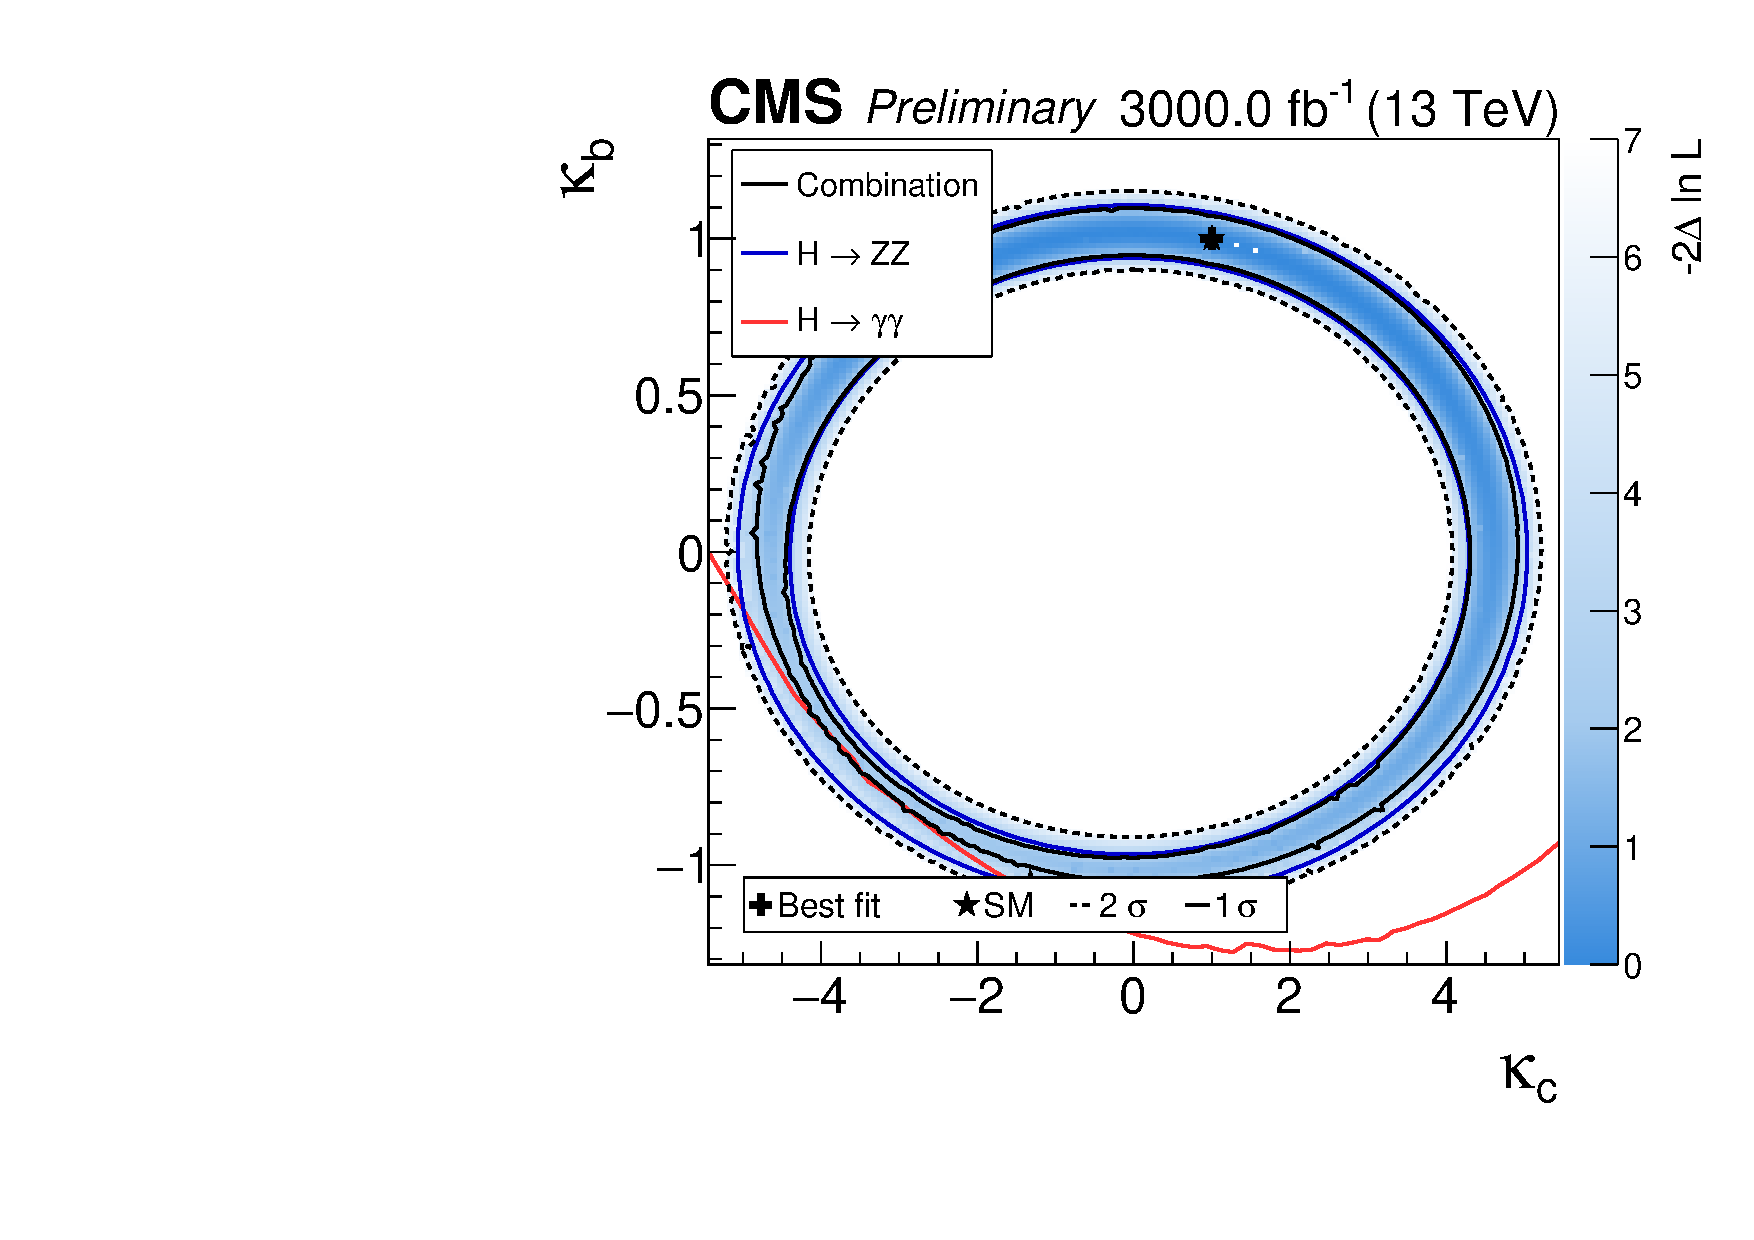
\includegraphics[width=0.49\linewidth]{img/projection_kbkc_plot_couplingdependentBRs.pdf}
    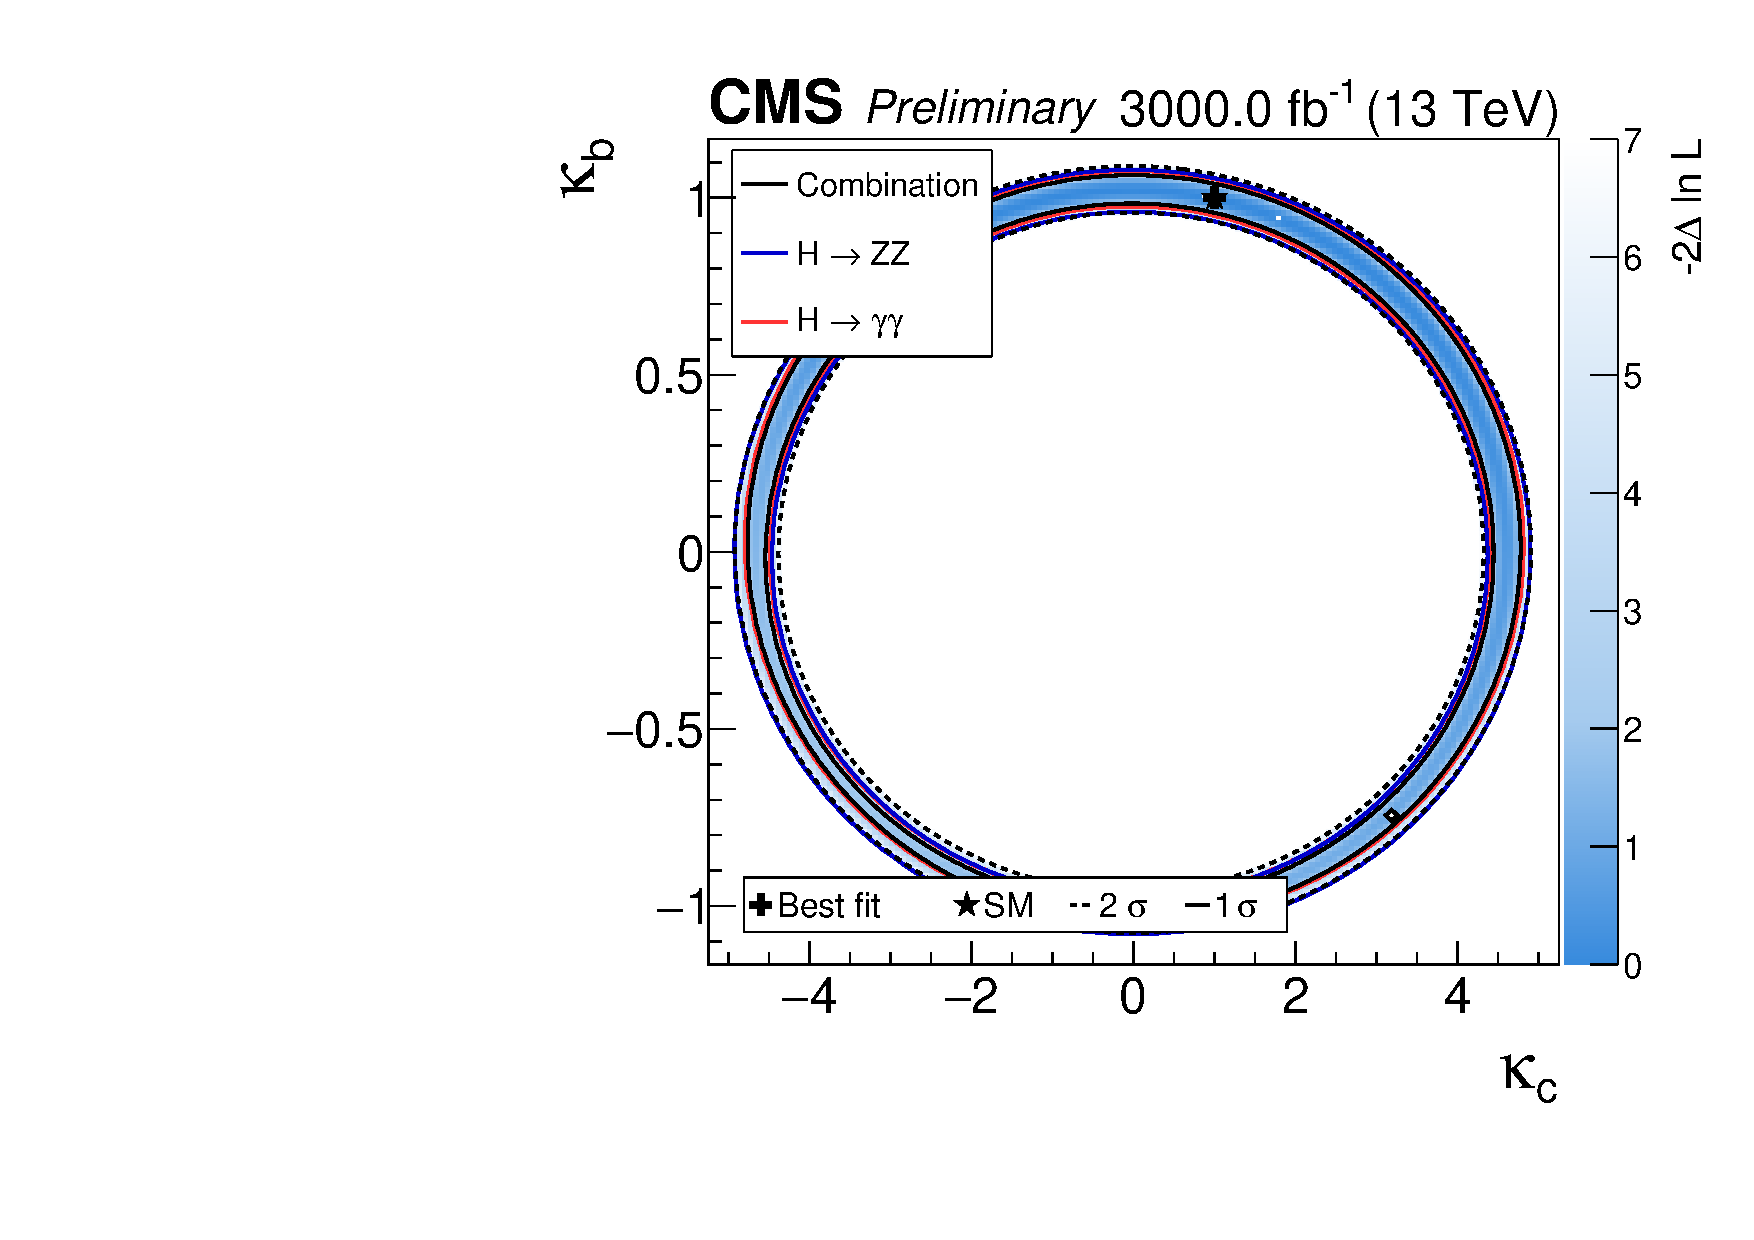
\includegraphics[width=0.49\linewidth]{img/projection_kbkc_plot_couplingdependentBRs_scenario2.pdf}
    % 
    \caption{
        Simultaneous fit to data for $\kappab$ and $\kappac$, assuming a coupling dependence of the branching fractions for Scenario 1 (\cmsLeft) and Scenario 2 (\cmsRight).
        % 
        The one standard deviation contour is drawn for the combination ($\hgg$ and $\hzz$), the $\hgg$ channel, and the $\hzz$ channel in black, red, and blue, respectively.
        % 
        For the combination the two standard deviation contour is drawn as a black dashed line, and the negative log-likelihood value on the coloured axis.
        }
    \label{fig:kbkc_couplingdependentBRs}
  \end{center}
\end{figure}

\begin{figure}[hbtp]
  \begin{center}
    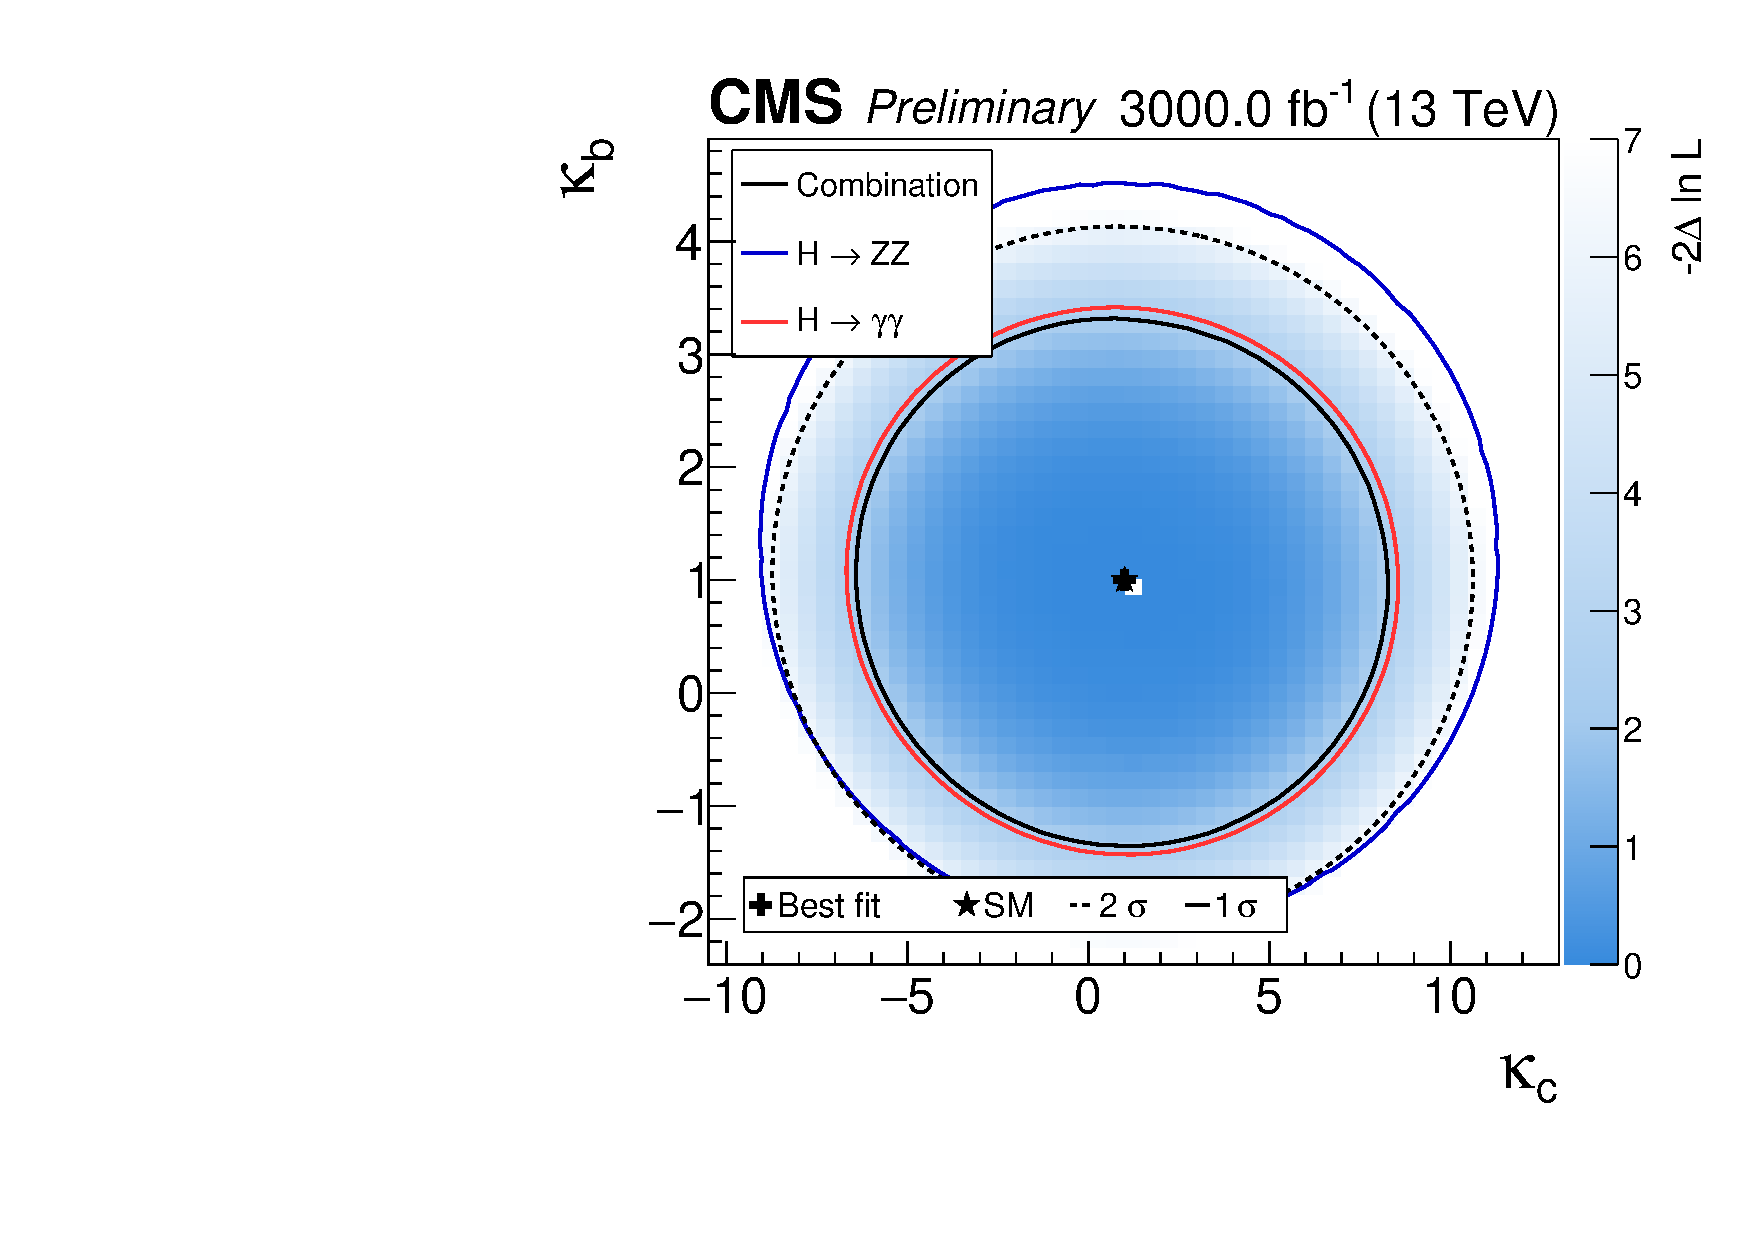
\includegraphics[width=0.49\linewidth]{img/projection_kbkc_plot_floatingBRs.pdf}
    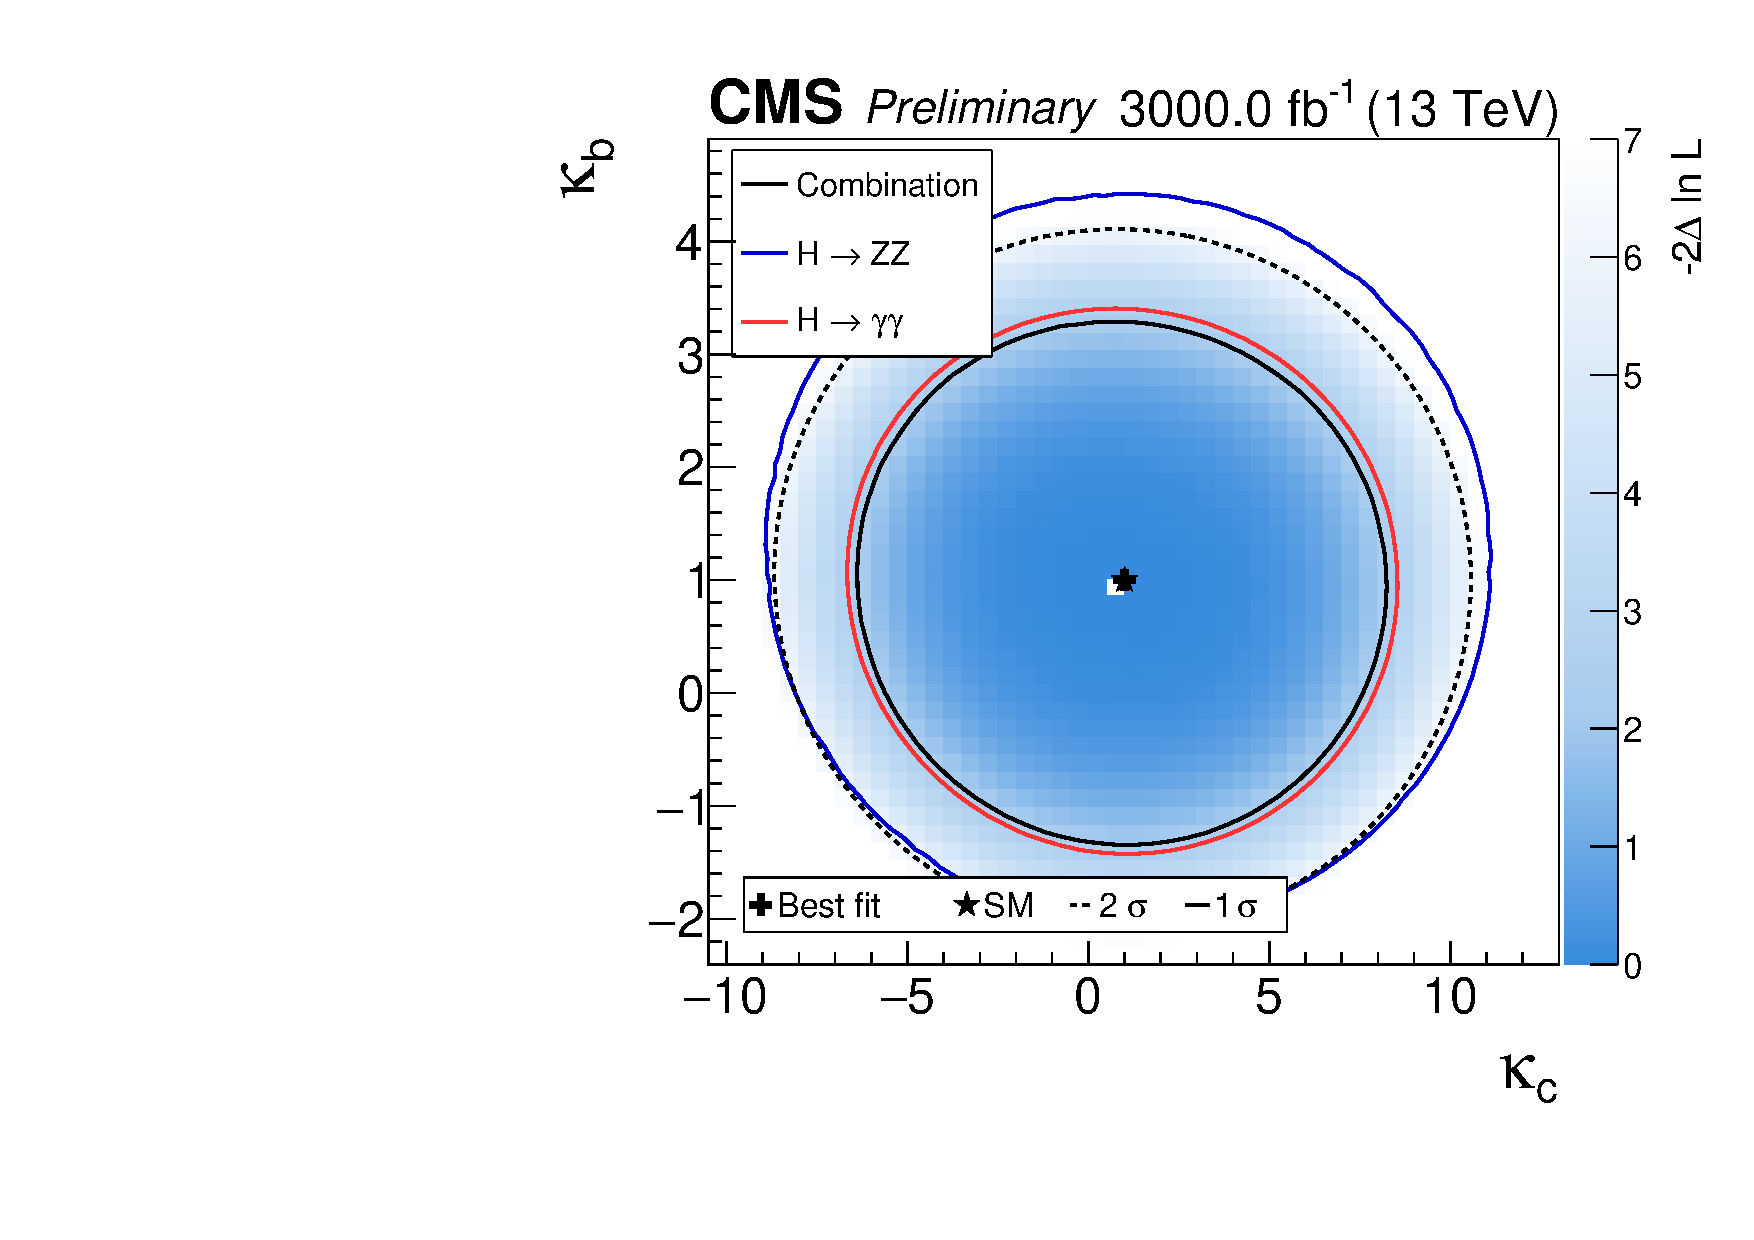
\includegraphics[width=0.49\linewidth]{img/projection_kbkc_plot_floatingBRs_scenario2.pdf}
    % 
    \caption{
        As Fig.~\ref{fig:kbkc_couplingdependentBRs}, but with the branching fractions implemented as nuisance parameters with no prior constraint.
        % 
        % Simultaneous fit to data for $\kappab$ and $\kappac$ with the branching fractions implemented as nuisance parameters with no prior constraint for Scenario 1 (\cmsLeft) and Scenario 2 (\cmsRight).
        % % 
        % The one standard deviation contour is drawn for the combination ($\hgg$ and $\hzz$), the $\hgg$ channel, and the $\hzz$ channel in black, red, and blue, respectively.
        % % 
        % For the combination the two standard deviation contour is drawn as a black dashed line, and the negative log-likelihood value on the coloured axis.
        }
    \label{fig:kbkc_floatingBRs}
  \end{center}
\end{figure}




\toggledclearpage 

% _______________________________________________________________________________________________
%% **DO NOT REMOVE BIBLIOGRAPHY**
\bibliography{auto_generated}   % will be created by the tdr script.

% ____________________________________________________________________________
%% examples of appendices. **DO NOT PUT \end{document} at the end
%\clearpage
\appendix

% \clearpage
% \input{tex/appendix_paper.tex}

% \clearpage
% \input{tex/appendix_scans.tex}

% \clearpage
% \input{tex/appendix_param_values.tex}

% \clearpage
% \input{tex/appendix_chi2_test.tex}

% \clearpage
% \input{tex/appendix_projections.tex}

% ____________________________________________________________________________
\clearpage

